\documentclass[a4paper]{article}

\usepackage{amsmath}
\usepackage{amsfonts}
\usepackage{graphicx}
\usepackage{enumerate}
\usepackage{hyperref}
\usepackage{anysize}
\usepackage{hyperref}
\usepackage{listings}
\usepackage{color}
\usepackage{tikz}

\marginsize{2.5cm}{2.5cm}{1.5cm}{1.5cm}
\setlength{\parindent}{0pt}

\graphicspath{{./images/}}

\usetikzlibrary{arrows, shapes}
\tikzstyle{arrow} = [->,font=\scriptsize,>=angle 90]
\tikzstyle{block} = [draw, rectangle, text width=12em, rounded corners, minimum height=2.5em, node distance=1.5cm]
\tikzstyle{cloud} = [draw, ellipse, text width=6em, text centered, minimum height=2.5em]
\tikzstyle{inner} = [inner sep=0, minimum size=0, node distance=1.5cm]

\title{P\&D Encryption---Final Report}
\author{Pieter Maene and Stijn Meul}
\date{\today}

\begin{document}
\lstset{
    language=C,
    numbers=left,
    stepnumber=1,
    numbersep=10pt,
    backgroundcolor=\color{white},
    showspaces=false,
    showstringspaces=false,
    showtabs=false,
    tabsize=2,
    captionpos=b,
    breaklines=true,
    xleftmargin=30pt,
    basicstyle=\footnotesize\ttfamily, 
    breakatwhitespace=true
}

\maketitle

\section{Overview}
In this report we discuss all the details of the P\&D project for multimedia and embedded systems. First a description of our application is given. All design decisions and the complete architecture are described. In the next part of this report more details about optimizations and the implementation of the application are given. Finally all issues and difficulties about porting the resulting algorithm to the DSP are given.

\section{Application Description}

The application consists of two main parts: the handshake and the encryption of data packets. For the handshake we use the STS protocol, while the encryption is based on AES-CTR. In this section, we will cover both of them in depth.

\subsection{Handshake}

\begin{figure}[h]
    \centering
    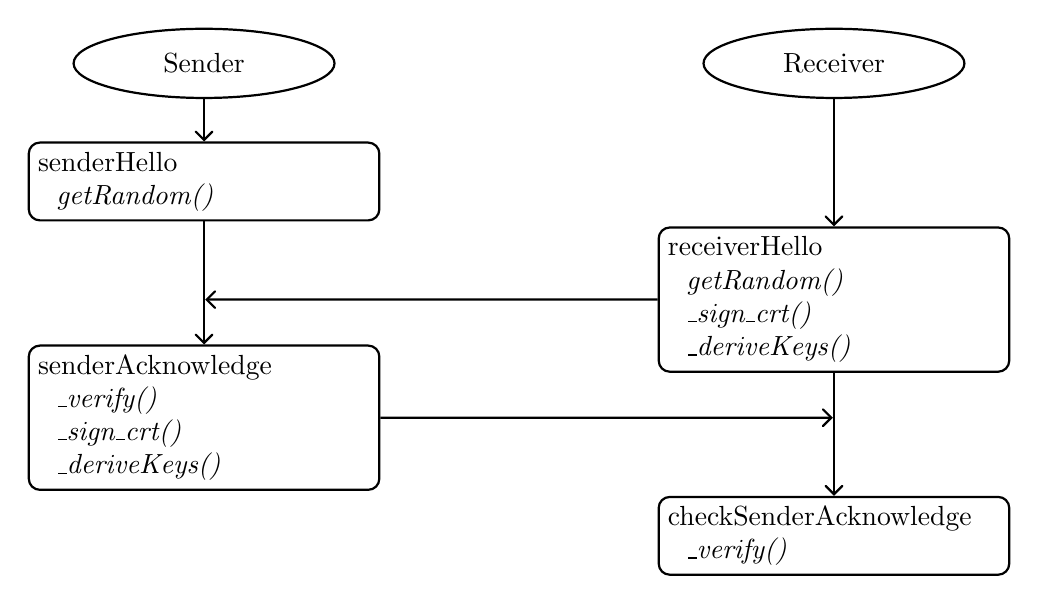
\begin{tikzpicture}[auto, node distance=8cm, thick]
        \node [cloud] (sender) {Sender};
        \node [block, below of=sender] (senderHello) {senderHello\\\textit{\ \ getRandom()}};
        \node [inner, below of=senderHello] (iSenderHello) {};
        \node [block, below of=iSenderHello] (senderAcknowledge) {senderAcknowledge\\\textit{\ \ \_verify()}\\\textit{\ \ \_sign\_crt()}\\\textit{\ \ \_deriveKeys()}};
        \node [cloud, right of=sender] (receiver) {Receiver};
        \node [block, below of=receiver, node distance=3cm] (receiverHello) {receiverHello\\\textit{\ \ getRandom()}\\\textit{\ \ \_sign\_crt()}\\\textit{\ \ \_deriveKeys()}};
        \node [inner, below of=receiverHello] (iReceiverHello) {};
        \node [block, below of=iReceiverHello] (checkSenderAcknowledge) {checkSenderAcknowledge\\\textit{\ \ \_verify()}};
        
        \path [arrow] (sender) edge (senderHello);
        \path [arrow] (receiver) edge (receiverHello);
        \path [arrow] (senderHello) edge (senderAcknowledge);
        \path [arrow] (receiverHello) edge (iSenderHello);
        \path [arrow] (receiverHello) edge (checkSenderAcknowledge);
        \path [arrow] (senderAcknowledge) edge (iReceiverHello);
    \end{tikzpicture}
    
    \caption{Handshake with Important Functions}
    \label{fig:handshake_with_functions}
\end{figure}

\subsubsection{Protocol Messages}

In the Station-to-Station protocol, three messages will be exchanged between the sender and receiver. After this three-way handshake both DSPs will have enough information to derice all necessary keys.

\begin{enumerate}
    \item The sender generates a random number $x$ and then sends $\alpha^x\ mod\ p$ to the receiver. This is shown in Table~\ref{tab:key_exchange_packet_senderhello}.
    \item The receiver generates a random number $y$ and sends $\alpha^y\ mod\ p$ to the sender. We then calculate the RSA signature of the concatenation of $\alpha^y\ mod\ p$ and $\alpha^x\ mod\ p$. This signature is then encrypted using the derived key and nonce. This is shown in Table~\ref{tab:key_exchange_packet_receiverhello}.
    \item The sender acknowledges the message from the receiver by sending its signature to the receiver, using the same procedure described previously. The only difference is that we now concatenate $\alpha^x\ mod\ p$ and $\alpha^y\ mod\ p$. This is shown in Table~\ref{tab:key_exchange_packet_senderacknowledge}.
    \item The receiver checks this final message and verifies the signature. This way, it is able to assert the sender has received correctly too.
\end{enumerate}

\begin{table}[H]
    \begin{center}
        \begin{tabular}{| c | c |}
            \hline
            TAG & KEY \\ \hline\hline
            1B & 156B \\ \hline
            0x00 & $\alpha^x\mod{p}$ \\
            \hline
        \end{tabular}
    \end{center}
    \
    \caption{Key Exchange Packet---SenderHello [Bytes]}
    \label{tab:key_exchange_packet_senderhello}
\end{table}
\begin{table}[H]
    \begin{center}
        \begin{tabular}{| c | c | c |}
            \hline
            TAG & KEY & SIGNATURE \\ \hline\hline
            1B & 156B & 20B \\ \hline
            0x01 & $\alpha^y\mod{p}$ & $\text{AES}_\text{K}\left(\left(\text{SHA-256}\left(\text{PKCS}\left(\alpha^y\small|\alpha^x\right)\right)\right)^{d_R}\mod{n_R}\right)$\\
            \hline
        \end{tabular}
    \end{center}
    
    \caption{Key Exchange Packet---ReceiverHello [Bytes]}
    \label{tab:key_exchange_packet_receiverhello}
\end{table}
\begin{table}[H]
    \begin{center}
        \begin{tabular}{| c | c |}
            \hline
            TAG & SIGNATURE \\ \hline\hline
            1B & 20B \\ \hline
            0x02 & $\text{AES}_\text{K}\left(\left(\text{SHA-256}\left(\text{PKCS}\left(\alpha^x \small|\alpha^y\right)\right)\right)^{d_S}\mod{n_S}\right)$\\
            \hline
        \end{tabular}
    \end{center}

    \caption{Key Exchange Packet---SenderAcknowledge [Bytes]}
    \label{tab:key_exchange_packet_senderacknowledge}
\end{table}

We decided to use SHA2 instead of SHA3 (which we chose in previous reports) because there is no standardised RSA padding scheme (like PKCS for SHA2) available yet for this hash function. We evualated our RSA implementation using a test vector provided by Mikhail Fomichev and Shayan Kaman Zadeh (Crypto 8).\\

This is a rather slow, mainly because there are a lot of modular exponentiations (both in calculating the Diffie-Hellman exponentions and the RSA Sign

\subsubsection{Signatures}

The calculation of an RSA signature is standardised in RFC3447. We implemented the RSASSA-PKCS1-v1\_5 algorithm, using SHA-256 to calculate the hash. Finally, the STS protocol requires us to encrypt the signature. For this we use AES in CTR mode with the derived key and nonce. The counter value is set to zero for this encryption.\\

We switched to SHA-256 instead of SHA-3 (which we chose in previous reports) because there is no standardised RSA padding scheme available yet for this hash function. We evaluated our RSA implementation using a test vector provided by Mikhail Fomichev and Shayan Kaman Zadeh (Crypto 8).

\subsection{Key Derivation}
\label{par:key_derivation}

After the key exchange is done, we can derive the two keys (a 128-bit AES key, an 80-bit HMAC key) and the 64-bit nonce used in the CTR block cipher mode (see Paragraph~\ref{par:data_encryption}). These derivations are obtained by calculating SHA-256 hashes of the shared key with a 1, 2 and 3 appended at the end. Finally, for each key the required number of bits is selected from the hash.

\subsection{Data Encryption}
\label{par:data_encryption}

Because of the realtime character of the application, it is not possible to use modes which introduce a dependency between blocks. This restriction is imposed because some blocks might get lost during transmission. In a speech application lost blocks are not really an obstacle as long as enough blocks still arive at the receiver.\\

The mean advantage of the CTR mode is the fact that it can be parallelised. To decrypt a block, you only need the nonce and the counter value. There are no other dependencies. This means that packets can be decrypted immediately after receiving them. Another advantage is that it only uses the AES encryption function for both encrypting and decrypting the data.

\begin{figure}[h]
    \centering
    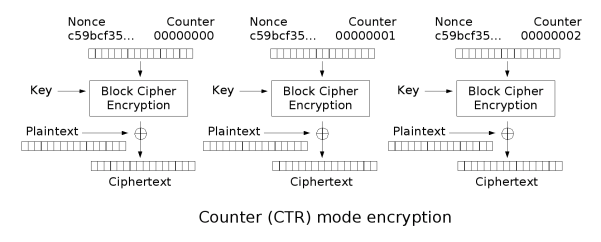
\includegraphics[scale=0.75]{ctr_encryption.png}
    \caption{CTR Encryption---Source: Wikipedia}
    \label{fig:ctr_encryption}
\end{figure}

In the final design, the input to the AES encryption function is given in Table~\ref{tab:ctr_mode_aes_encryption_input}. As we saw in Paragraph~\ref{par:key_derivation}, the 64-bit nonce is derived from the shared key. Furthermore, we actually have two counter: one for the packets and for the blocks inside this packet. The former denotes the current packet and is transmitted along with the data (see Table~\ref{tab:data_packet}). We take care to restart the handshake when this counter wraps around. This is necessary, because otherwise if a repeat of a given plaintext would result in the same ciphertext. The latter is required because each plaintext block can only be 128 bits long. To encrypt larger packets, we need this second counter value to have a unique encryption result.

\begin{table}[H]
    \begin{center}
        \begin{tabular}{| c | c | c |}
            \hline
            Nonce & Packet Counter & Block Counter \\ \hline
            8B & 4B & 4B \\
            \hline
        \end{tabular}
    \end{center}

    \caption{CTR Mode---AES Encryption Input [Bytes]}
    \label{tab:ctr_mode_aes_encryption_input}
\end{table}
\begin{table}[H]
    \begin{center}
        \begin{tabular}{| c | c | c | c | c |}
            \hline
            TAG & COUNTER & DATA & HMAC \\ \hline
            1B & 4B & 128B & 20B \\
            \hline
        \end{tabular}
    \end{center}
    
    \caption{Data Packet}
    \label{tab:data_packet}
\end{table}

\subsection{HMAC}

The authenticity of a data packet is asserted using an HMAC. This code is based on keyed-hash messages and is standardised in FIPS 198-1. We again use SHA-256 to calculate the hashes, which is one of the approved functions by NIST. We chose to use an HMAC because it allows for secure and fast message authentication.

\section{Optimizations}

\subsection{Optimization Table}

\begin{center}
    \begin{tabular}{| l | c | r |}
        \hline
        Code Stage & Number of Cycles & Code Gain \\ \hline
        Base Code & $6,20662313 \cdot 10^{8}$ 	& $0\%$ \\
        CRT Optimization & $4,35591090 \cdot 10^{8}$ & $29,82\%$ \\
        USE64WITH32 Optimization 	& $4,29177952 \cdot 10^{8}$ & $1,03\%$ \\
        Optimization of Conversion Functions & $4,24002677 \cdot 10^{8}$ & $0,83\%$ \\
        Restrict Optimization	 & $1,80351722 \cdot 10^{8}$ & $39,26\%$ \\
        \hline
    \end{tabular}
\end{center}

\subsection{CRT Optimization}
The implementation of the Chinese Remainder Theorem is an algorithmic optimization and not a DSP specific one.\\

The Chinese Remainder Theorem uses the fact that both prime numbers $p$ and $q$ are known. This gives the possibility to calculate two seperate exponentiations of half the length of the original one. In theory this would make the exponentiation four times faster. As both results need to be recombined again, the practical implementation is a little slower.\\

For the practical implementation Garner's algorithm is used. As both exponentiations have no data dependencies, they can be parallelized completely. To show this parallelization practically, we have implemented these two exponentiations using pthreads on CentOS. As the OMAP-L138 board does not have an OS which is supporting threads this is more difficult to implement on the board. If the ARM processor could be used as well, it would be possible to do one exponentiation on the DSP and another one on the DSP. \\

It should also be noted that the given Diffie⁻Hellman parameters are a faster sub-group from what could be given. This should be taken into account when evaluating the cycle count as with other parameters the execution time would increase.

\subsection{USE64WITH32 Optimization}
USE64\_WITH32 is a $\#$define statement in the BigDigits library we are using. If this switch is activated, 64-bit behavior is simulated in 32-bit environment in C.

\subsubsection{Example}
When the USE\_64WITH32 flag is set the following code is called for the multiply function. The performance gain can be seen as there is no seperate code to do the transfer of carry bits from one 32-bit variable to another.

\lstinputlisting[language=C]{source/use64.c}

\subsubsection{Impact of the Optimization}
The impact of this optimization is quite large as the multiply function is called many times during the handshake. This gives an optimization of $1,85071223\cdot10^{8}$ cycles.

\subsection{Optimization of Conversion Functions}
This optimization is more an improvement of our code than a real DSP optimization. The optimization was applied in the handshake functions of the code located in protocol.c.\\

All the contents of the \textbf{field\_t} type (the type we use for packets) are passed as char types even if the functions in the bigdigits library require a digit\_t as input. Before the conversion optimization all these digit\_t variables were first converted from digits to chars using the mpConvToOctets() function in the bigdigits library. The next function in the handshake then reconverted all these chars to \textbf{digit\_t} types using \textit{mpConvFromOctets()} so they could be used by the bigdigits library.\\

This conversion and reconversion of these large variables are not only cumbersome for the calculation time, they are also very inefficient in memory usage as each average pointer variable is around 150 bytes long and each conversion required a temporary variable as a destination for the conversion.\\

The optimization is just a cast of the \textbf{digit\_t} variable to a char so it can be added to the packet of type \textbf{field\_t}. The bytes are then interpreted incorrectly but this is of no importance as they are casted back to \textbf{digit\_t} before they are used again.

\subsubsection{Example}
The following C snippet demonstrates the \textit{senderHello()} function before the optimization:
\lstinputlisting[language=C]{source/senderHelloNoOptimization.c}
The following C snippet demonstrates the \textit{senderHello()} function after the optimization:
\lstinputlisting[language=C]{source/senderHelloConversionOptimization.c}

\subsubsection{Impact of the Optimization}
The conversion optimization gives a saving of $5,175275\cdot10^{6}$ cycles. Again this gain in cycles is this great because of the length of the variables. Also the memory usage is more efficient as we save a lot of temporary variables.

\subsection{Restrict Optimization}

The addition of the \textbf{restrict} keyword to all our pointer variables is an intrinsic DSP optimization.

\subsubsection{Example}
The only changes that need to be made to implement the restrict optimization is adding the restrict keyword in front of all the pointer arguments in the function headers. An example of a function header with the restric keyword:

\lstinputlisting[language=C]{source/restrictheader.c}
An example of the same function header before the restrict optimization:

\lstinputlisting[language=C]{source/norestrictheader.c}

\subsubsection{Impact of the Optimization}
When the compiler is compiling code with a lot of pointer arguments, it is being very pessimistic about the content of the pointer arguments. For the compiler it is much safer to suppose all the contents of the pointer are changed during the function call except that in most implementations this assumption is too strong. When adding the restrict keyword in front of pointer arguments, the compiler supposes that only the current function is altering the values of the pointer. By doing so the compiler is able to parallelize most of the copying from and to that variable which gives a great improvement.\\

As the average pointer variable in our code has a length of approximately 150 bytes, this optimization results in a much faster execution time. $2,43650955\cdot10^{8}$ cycles are saved by implementing this DSP optimization.

\section{Porting and Integration}

\subsection{Porting from Linux to CCS}
One of the errors we encountered during the porting from Linux to CCS was that the length of arrays need to be a constant. This was quickly solved as the variable length we used in some functions was just to make our code easy to customize. Overall the same lengths were used throughout the code, so they could be easily replaced by constants.

\subsection{Integration with Speech}
Integration with the speech group went very fluently as we already foresaw possible issues. To simplify integration with the speech group, we implemented a shared buffer and a modified flag. Every time a variable is written to this shared buffer, the modified flag is set to true. Every time a variable is read from the shared buffer, this modified flag is set back to false. In this way, we (=the crypto group) know when we can read the next data sequence from speech to start encrypting. The speech group knows when their last packet is read out for encryption when the modified flag is set to false.\\

Another parameter that needed to be checked was that the SRAM was still large enough to combine the code of both groups.

\subsection{Porting from CCS to the Board}
Porting our seperate code from CSS to the Board was not very difficult. When our code was combined with the code of the speech group, porting became more of a challenge as we encountered some memory issues. Apparently the memory size of both codes was too big to fit in SRAM. After a long and hard day of debugging the conclusion was that our providence striked back as the buffer size was unrealisticly high to fit on the DSP. After changing these buffer sizes to the minimum needed for the speech group, everything worked correctly.

\section{Load Double Word Optimization}
The double word optimization was another optimization we tried to implement but did not give any significant improvements.

\subsection{Example}
\lstinputlisting[language=C]{source/nassert.c}

\subsection{The Reason for Not Implementing}
The reason we did not implement this is because of the \textbf{DATA\_ALIGN} pragma which can not be defined on a function level. As an attentive reader would remark the previous code snippet will give compilation errors as the pragma does not recognize the \textit{encryptedData} variable which is only defined on function level. As it would be too cumbersome for us as programmers to keep track of all our variables as they would be defined globally we chose not to implement this optimization.

\section{Lessons Learnt}
One of the more important lessons we have learned is that implementing an algorithm on an embedded system is not just writing some C code. For an embedded system the challenge only starts when the code is functioning correctly. Although our code did not lent itself for loop optimizations as the speechcode did, still a lot of improvement could be made by giving the compiler some hints for optimizations.\\

Another very important lesson we learned is that compilers are already pretty good at optimizing code. In our quest for optimizations we never managed to achieve a better compilation time than the compiler could with level two optimizations enabled. \\

Although compilers are already quite smart, some optimizations like the \textbf{restrict} keyword can never be achieved by a compiler on its own. The knowledge of the algorithm together with the compilers optimization knowledge are the road to a fast execution time.\\

A final very important lesson is although the code of both teams is working correctly on its own, it does not guarantee a correct functioning system. Of course the rule of thumb in engineering is that it is always the other team's responsibility...

\section{Conclusions}

\end{document}
